% ---------------------------------------------------
% ----- Main document of the template
% ----- for Bachelor-, Master thesis and class papers
% ---------------------------------------------------
%  Created by Claudia Müller-Birn on 2012-08-17. (last update 2015-10-20)
%  Freie Universität Berlin, Institute of Computer Science, Human Centered Computing (HCC).
%
\documentclass[pdftex,a4paper,11pt]{scrartcl}
%
%---------------------------------------------------
%----- Packages
%---------------------------------------------------
%
\usepackage[T1]{fontenc}
\usepackage[utf8]{inputenc}
%\usepackage[ngerman]{babel}
\usepackage[english]{babel}
\usepackage{ae}
\usepackage{bibgerm}

\usepackage{fancyref}
\usepackage{fancyhdr} % Define simple headings
\usepackage{xcolor}
\usepackage{url}
\usepackage{verbatim}
%
\usepackage[pdftex]{graphicx}
\usepackage{hyperref} % turn all your internal references into hyperlinks
%\usepackage[pdfstartview=FitH,pdftitle={<<Titel der Arbeit>>}, pdfauthor={<<Autor>>}, pdfkeywords={<<Schlüsselwörter>>}, pdfsubject={<<Titel der Arbeit>>}, colorlinks=true, linkcolor=black, citecolor=black, urlcolor=black, hypertexnames=false, bookmarksnumbered=true, bookmarksopen=true, pdfborder = {0 0 0}]{hyperref}
%
% a new command is defined that allows to include an empty page when needed
\newcommand{\blankpage}{
\newpage
\thispagestyle{empty}
\mbox{}
\newpage
}
%
%---------------------------------------------------
%----- PDF and document setup
%---------------------------------------------------
%
\hypersetup{
	pdftitle={<My title>},  % please, add the title of your thesis
    pdfauthor={<Author>},   % please, add your name
    pdfsubject={<<Bachelor/Master thesis>, Institute of Computer Science, Freie Universität Berlin>}, % please, select the type of this document
    pdfstartview={FitH},    % fits the width of the page to the window
    pdfnewwindow=true, 		% links in new window
    colorlinks=false,  		% false: boxed links; true: colored links
    linkcolor=red,          % color of internal links
    citecolor=green,        % color of links to bibliography
    filecolor=magenta,      % color of file links
    urlcolor=cyan           % color of external links
}
%
%---------------------------------------------------
%----- Settings for word separation
%---------------------------------------------------
% Help for separation (from package babel, section 22)):
% In german package the following hints are additionally available:
% "- = an explicit hyphen sign, allowing hyphenation in the rest of the word
% "| = disable ligature at this position. (e.g., Schaf"|fell)
% "~ = for a compound word mark without a breakpoint (e.g., bergauf und "~ab)
% "= = for a compound word mark with a breakpoint, allowing hyphenation in the composing words
% "" = like "-, but producing no hyphen sign (e.g., und/""oder)
%
% Describe separation hints here:
\hyphenation{
% Pro-to-koll-in-stan-zen
% Ma-na-ge-ment  Netz-werk-ele-men-ten
% Netz-werk Netz-werk-re-ser-vie-rung
% Netz-werk-adap-ter Fein-ju-stier-ung
% Da-ten-strom-spe-zi-fi-ka-tion Pa-ket-rumpf
% Kon-troll-in-stanz
}

%---------------------------------------------------
%----- Settings for title page
%---------------------------------------------------

\begin{titlepage}

\title{\includegraphics[width=0.6\textwidth]{pics/FU_logo.pdf}\\
{\small <Bachelor-/Masterarbeit> am Institut für Informatik der Freien Universität Berlin}\\
{\small Human-Centered Computing (HCC)}\\
[6ex]
{\LARGE<Titel der Arbeit>}\\
{\normalsize-- Exposé --}}

\author{
{\emph{\normalsize<Ihr Vor- und Nachname>}}\\
{\normalsize Matrikelnummer: <IhreMatrikelnummer>}\\
{\normalsize <ihreemail@adresse.de>}\\\\
{\normalsize Betreuerin: Prof. Dr. C. Müller-Birn}
}

\date{\normalsize Berlin, <Datum>}

\end{titlepage}

%%%%%%%%%%%%%%%%%%%%%%%%%%%%%%%%%%%%%%%%%%%%%%%%%%%%%%
% The content part of this document starts here! %%
%%%%%%%%%%%%%%%%%%%%%%%%%%%%%%%%%%%%%%%%%%%%%%%%%%%%%%

\begin{document}

\maketitle

\thispagestyle{empty}  % remove page number on the title page

\blankpage

%---------------------------------------------------
%----- Content part
%---------------------------------------------------
\setcounter{page}{1} % page number is set to "1" otherwise it would be "3"

\section{Motivation}
%\noindent \emph{In welchem Bereich/Themenfeld bewegt sich Ihre geplante Arbeit? }

This thesis is situated in the field of human-computer interaction and more specifically algorithmic governance and socio-technical systems.
Algorithmic governance refers to the notion of algorithms used in governance systems, (partially) taking decisions concerning humans.
As Danaher et al. put it ``algorithms are increasingly being used to nudge, bias, guide, provoke, control, manipulate and constrain human behaviour''~\cite{DanaherEtAl2017}.
%TODO: def!

Wikipedia is a complex socio-technical system where mechanisms of algorithmic governance are increasingly used.
Unlike many others, it is also an open socio-technical system that allows us to study phenomena we can't observe elsewhere.
Since its birth in 2001, the free online encyclopedia has come to comprise nearly 300 different language versions and 48,364,313 articles (\url{https://en.wikipedia.org/wiki/List_of_Wikipedias}, accessed: July 23rd, 2018).
Today, nearly 2000 bots exist in Wikipedia which perform various tasks regarding community support and maintenance.
At the latest when there are users who are not sure anymore whether they interact with a human user or a bot~\cite{FordGeiger2012}, it is time to evaluate critically the automated agents active in the system.
How are these automated systems influencing the Wikipedian community?
Are there bots that implement hard rules ("Code is law") that nobody intended to have but end up in there anyway?

%TODO: Bots def


\section{Literature Review}
%\subsection{Thematische Einordung}

Following literature was so far identified as relevant for the present thesis:

\subsection{Algorithms/algorithmic governance}

\cite{DanaherEtAl2017}
  %title = {Algorithmic governance: Developing a research agenda through the power of collective intelligence},
Danaher et al.~\cite{DanaherEtAl2017} propose a framework for researching algorithmic governance systems, their effectiveness and legitimacy.
They provide a ``detailed map of key research themes, questions and methods'' which seems to be particularly useful for the current research proposal.

\cite{BarHooZie2013}
%title={Governing algorithms: A provocation piece},
"Tarleton Gillespie identifies six dimensions of what he
termed “public relevance algorithms”:
“patterns of inclusion,” // how about patterns of exclusion?
“cycles of anticipation,”
“the evaluation of relevance,” 
“the promise of algorithmic objectivity,”
“entanglement with practice,”
and “the production of calculated publics” (Gillespie forthcoming)."

the specificity question:
algorithm = computer = software = machine = god?

distinction algorithms/data:
"This upends the common notion that access to the source code of
software grants full access to the software’s functionality."

delegating knowledge production to machines: met with fierce resistance

2 types of automation tasks delegated to machines
- subjecting data to analysis, tasks impossible to perform manually
- decision making

agency and control: who's the arbiter? who excercises control/autority over the
algorithm?

deferral of accountability:
"Similar to invocations of
“technical failure,” responsibility and blame tend to be put on “the
algorithm”."

people are often unaware of where algorithms are at work (siehe zb Writing up
paper where a Wikipedia editor wasn't sure whether it was a bot or a person who
was deleting their contributions)
Who understands the algorithms:
"But even if these algorithms
were somehow more manifest, would we find that they are nonetheless
inscrutable?"
secrecy: trade secret, blabla
legal issues


\subsection{Bots on Wikipedia}
\cite{Geiger2017}
%title = {Beyond opening up the black box: Investigating the role of algorithmic systems in Wikipedian organizational culture},
- describes complex interplay between social and technical systems in governing wikipedia

  Geiger~\cite{Geiger2017} is just one example of numerous works on the societal implications of bots and algorithmic systems in general in Wikipedia's ecosystem.
  It addresses various aspects and consequences of algorithmic governance within Wikipedia, such as driving away newcomers through an overly complicated bureaucratic process which results in Wikipedia turning into a gated community where only experienced users can fully participate.

"Wikipedia demonstrates how the issues in and around
algorithmic systems are as much social as they are tech-
nical, going far beyond the opacities that arise around
proprietary source code. My argument extends Burrell’s
(2016) discussion of three different forms of opacity in
machine learning: intentional secrecy (proprietary
source code), technical literacy (such as learning to
read code), and opacities inherent in machine learning
(such as issues of interpretability). To these forms, I add
another: the opacities in learning a particular institu-
tional or organizational culture that is supported by
algorithmic systems."
// source is open, but who can actually read it? and is willing to invest the time and energy in order to hold the system accountable?
// vgl auch Gedanke von Claudia: "Wikipedia is spannend, weil wir daran das erforschen können, was wir an Facebook nicht können. Und weil die ein Abbild der Gesellschaft im Kleinen ist."
// vgl auch Web Science def: observe micro behaviours in order to study macro phenomenons (governance, ..)

Requirements/Expectations for bot developers:
"bot developers are generally expected to be responsive
to reasonable requests and concerns from the
community."

"Wikipedians discuss and debate
about what kinds of bots should exist in the project,"

\cite{GeiHal2017}
- replication study of the paper "Even Good Bots Fight" that raised the theory
  that bots get into conflict/revert wars constantly
- introduce a very detailed open methodology, have a github and .. repository
  with their whole data processing pipeline
- operationalise conflict
- generate a data set
- analyse edit summaries, cluster bot activities accordingly
- 2 metrics: number of bot-pair-per-article reverts, time between reverts
- quantitative and qualitative analysis
- conclusion: only 0.something of all bot-bot-reverts are genuine conflict

trace ethnography: "seek to understand data in the context it has within a community of practice," "data to be a starting point for further contextualization and interpretation,"
operationalise conflict!
distinguish conflict from non-conflict in bot reverts
compile data set + meta data
background: wikipedia researchers + long-time contributors
findings: overwhelming majority of the reverts are routine collaborative work between bots
metrics: time between reverts; number of reverts per article for the same bot pair
in addition: in depth analysis of random examples from different parts of the statistical distribution of the metrics
classify patterns in edit summaries

research question: "to what extent are bot-bot reverts
in Wikipedia genuine conflicts where disagreements about how Wikipedia ought to be written were
embedded in opposing bot codebases, versus cases like Shoreland’s Addbot that reflect the opposite?"

\cite{HalKitRied2011}
Don't bite the newbies

\cite{MuellerBirn2014}
  Mueller-Birn et al.~\cite{MuellerBirn2014} provide an overview over different tasks bots in Wikipedia carry out.
  They categorise these in two main groups: community services and guidelines/policies.
  The authors also suggest that attitudes towards bots have changed over time, and acceptance of bots has gradually grown.


\subsection{Methodology}
\cite{GeiRib2011}
- define the trace ethnography methodology
- traditional ethnography + heavy reliance on documentation
- related to ANT
- idea: reverse documentation traces to reconstruct the story (what happened
  there)
- ethical concerns: people couldn't have consented in an informed manner


\section{Aim of the thesis}
%\noindent \emph{Welche Ziele werden mit der Arbeit verfolgt? Welche zentralen Fragen lassen sich daraus ableiten?}
The purpose of this thesis is investigating the translation of social into algorithmic rules on Wikipedia.
To this end, I will evaluate the community engagement of bots and try to understand which social norms in particular they intend to implement.
I am especially looking for cases in which there is a mismatch between what the bot is actually doing, what the developer intended it to do and what the community consensus was.
This would signify that bots have ended up implementing guidelines and norms in distorted way, effectively creating constraints that no one wanted to have to begin with and turning them into the status quo.
Furthermore, an analysis of established bot development frameworks such as pywikibot (\url{https://www.mediawiki.org/wiki/Manual:Pywikibot}), wikitools (\url{https://github.com/alexz-enwp/wikitools}) or Apibot (\url{apibot.zavinagi.org}) and their influence on prevalence of automated tasks is planned.
Finally, I'd like to also propose recommendations for ethical code guidelines for developing algorithmic systems which could be included in bot development frameworks.

\section{Planned procedure}

Following steps are planned in order to answer the research question(s):

\begin{itemize}
    \item assemble bots from different language versions (EN; DE; BG; ES; CAT); following resources can be useful to identify bots: the Bot user group; user\_former\_groups for former bots; "Bot user" cross-wiki category (\url{https://de.wikipedia.org/wiki/Wikipedia:Bots}); Wikidata Item “Q3681760”
    \item identify bots for which source code is available: consult the user page of the bots
    \item of the bots for which the source code is available: take exemplary cases paticularly active in the community sphere, and study their social context: what community norms do they try to implement? what discussions happened prior to implementing the bots?
    \begin{itemize}
        \item look at community pages concerning these bots: start at Village Pump (\url{https://en.wikipedia.org/wiki/Wikipedia:Village_pump})
        \item Request for Approval of the bot and corresponding discussions
    \end{itemize}
    \item study source code of the bots of interest: are there such that seem to contradict a policy or the consensus which lead to their implementation?
    \item contact bot operators and via them get in touch with the developer (mostly the same person); interview bot developers to better understand their motives and considerations while developing the bots
    \item look at bot frameworks (pywikibot, nochwas?): is there a disproportional emphasis on bot activities for which source code is provided in these frameworks where as other tasks get neglected?
    \item based on the insights won during described analysis, formulate ethical code recommendations
    \item familiarise yourself with existing bot policies; following Wikipedia resources can be of interest:
    \begin{itemize}
        \item \url{https://en.wikipedia.org/wiki/Wikipedia:Bot_Approvals_Group}
        \item \url{https://en.wikipedia.org/wiki/Wikipedia:Bot_policy}
        \item \url{https://en.wikipedia.org/wiki/Wikipedia:Bots/Requests_for_approval}
    \end{itemize}
\end{itemize}

I am also considering proposing a bot in front of the Bot Approval Group in order to gather better understanding for the social processes at work.
For this, following resource is of interest: \url{https://www.mediawiki.org/wiki/Manual:Creating_a_bot}.

\subsection{Bots}

This is a preliminary list of potentially interesting bots to look into:

\begin{itemize}
  \item HagermanBot (EN): signs unsigned discussion entries -- there was a
  controversy, because some users specifically didn't want their posts to be
  signed~\cite{MueDoHer2013}. % Eigtl Lives of Bots by Geiger, hab ich aber noch nicht gelesen
  \item CopperBot: German version of the HagermanBot
  \item AvicBot: moves pages from category A to category B, if merge request exist on Categories for Discussion, or removes a category entirely if the request is to empty the category
  \item CSDWarnBot: warns users when pages they've created are nominated for speedy deletion
  \item Mr.Z-bot: notifies users directly for users that are most likely spammers
  \item ClueBot NG + HBC AIV Helperbots and MartinBot: help fighting vandalism
  \item GiftBot (DE): removes processed flagged revision requests, disseminates a newsletter with new edits on pages
  \item xqbot (DE): has over 10 tasks listed on the German bot list overview page (\url{https://de.wikipedia.org/wiki/Wikipedia:Bots/Liste_der_Bots}), including fixing double redirects and interwiki links between different language versions, validating the voting rights of users during different surveys or administrator elections
%  \item What about the bots that tweet about anonyme edits from inside the Parliament/Congress/Bundestag?
\end{itemize}


\section{Methodological implementation}
%\noindent \emph{Mit welcher Methodik setzen Sie die einzelnen Aktivitäten in Ihrer Arbeit um?}
Regarding methodology, the present work is part( is situated/located at?) of the data/community analytics field/domain/area/scope/sphere.

% Trace ethnography
I will work with different types of quantitative and qualitative data, following closely the concept/methodology of trace ethnography~\cite{GeiRib2011} which also the excellent work of Geiger and Halfaker~\cite{GeiHal2017} implements.
%TODO: genaueres zu trace ethnography.
% "cooking data with care", also data science pipeline

Subtasks of the research involve source code analysis, document analysis and developer interviews.

\begin{comment}
  * what is the question and what are adequate methods to answer it?
  * GeiHal2017 haben einen "Epistemology Overview" chapter!
  * hauptsache: sich selber kritisch hinterfragen

* methods:
  * begin with some data dumps, but ask additional questions and supplement with different data and methods
  * cooking data with care: take note of data science pipeline: explore the data, compile it carefully, ask critical questions
  * interviews with bot developers: understanding their considerations when developing the bot code.
\end{comment}

% ANT
Furthermore, in order to identify the connections/interdependencies between different artefacts, people and events, I plan to draw upon some of the concepts and methods from the Actor-Network-Theory~\cite{Latour2010}, particularly on the mappings of controversies proposed by~\cite{Venturini2010a}.
The ANT is a model of redistributing actions and power.
Everyone and everything who does something (inter\emph{act} with something/somebody else) can be conceptualised as an actor: people, organisations, even objects.
According to the granularity and focus of observation, using ANT a researcher can zoom in and out in the network: every actor can be decomposed into a network and every network can be compressed into a single actor.
Venturini's proposal to map these multiple levels is particularly useful in order to characterise conflicts and controversies.

\section{Technical tools}
%\noindent \emph{Mit welchen softwaretechnischen Hilfsmitteln soll die Arbeit realisiert werden?}

I am planning on using following technical resources in order to realise afore mentioned steps:

\begin{itemize}
    \item python: for gathering, cleaning and analysing data automatically
    \item python + matplotlib, R and gnuplot: for charts and visualisations
    \item yEd (graph visualisation tool): for mapping controversies according to ANT
    \item audacity + transcriber: for recording and transcribing interviews with developers, in case they are conducted in person or via the phone
    \item maybe a tool for static source code analysis
\end{itemize}

\section{Some important definitions}

\subsection{Algorithm and algorithmic}
Def "algorithmic": "as involving encoded proced-
ures, which are typically—but not exclusively—compu-
tationally implemented."~\cite{Geiger2017}
% algorithm -- was ist der Unterschied zwischen Bot und Algorithmus

\subsection{Bot}
siehe GeiHal2017

\subsection{Algorithmic governance}

\subsection{Conflict}

\section{Preliminary schedule}
%\noindent  \emph{Wie ist der generelle Zeitplan der Arbeit? }

\begin{figure}[!h]
	\centering
		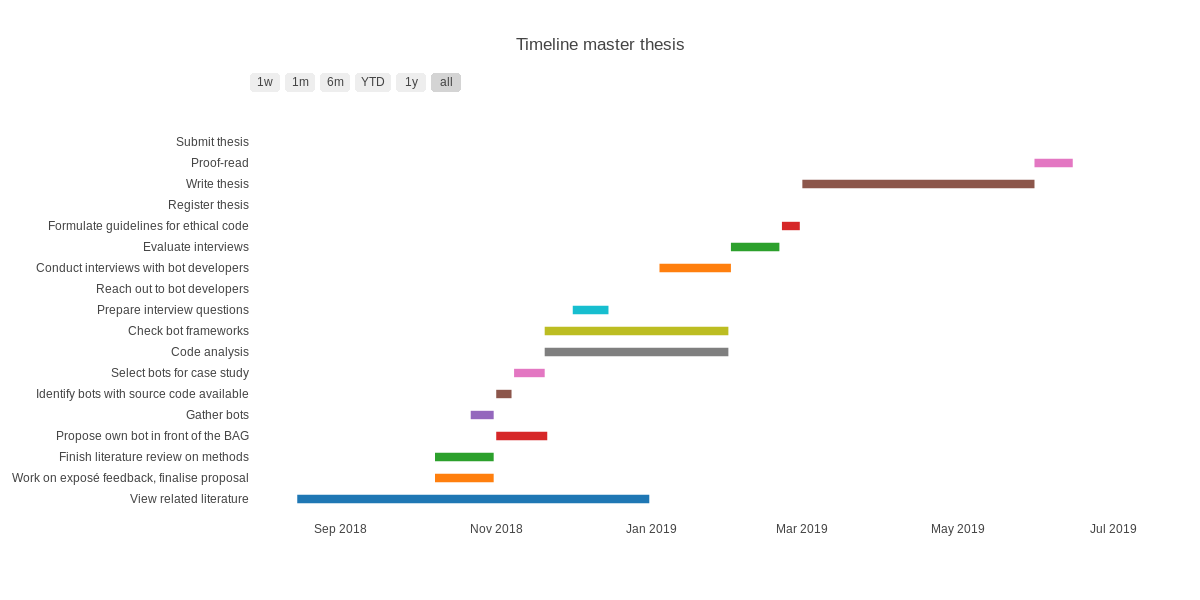
\includegraphics[width=1\textwidth]{../charts/gantt-thesis.png}
    \caption{Gantt chart timeline. There is a local interactive version of this chart so it is actually useful}
\end{figure}

\begin{tabular}{r p{11cm}}
    Aug 2018 - Sep 2018 & identify interesting bots; literature review; draft exposé \\
           Oct 2018 & present exposé; work on exposé feedback, finalise proposal;\\
    Nov 2018 - Dec 2018 & gather and analyse bot data: identify bots for the case studies, start code analysis, reach out to developers \\
           Jan 2019 & register the thesis with the Prüfungsbüro \\
Jan 2019 - Feb 2019 & finish work on code analysis and developer interviews \\
           Mar 2019 & start writing \\
           Jun 2019 & submit thesis \\
\end{tabular}

%---------------------------------------------------
%----- Bibliography
%---------------------------------------------------
\phantomsection
\addcontentsline{toc}{chapter}{Literatur}   % headline
\bibliographystyle{alpha}  % citation style
\bibliography{bibliography} % bib file


%---------------------------------------------------
%----- Appendices
%---------------------------------------------------
\begin{comment}
\newpage
\section*{Anhang I: Auszug Prüfungsordnung Master}
\label{sec:master}

\begin{figure}[!h]
	\centering
		\includegraphics[width=0.8\textwidth]{pics/Auszug_Master_Pruefungsordnung.pdf}
	\caption{Auszug Prüfungsordnung Master}
\end{figure}
\end{comment}

\end{document}
